\documentclass[border=6pt,12pt]{standalone}
\usepackage{times}
\usepackage{amsmath,amssymb}
\DeclareMathSizes{12}{12}{10}{8}   % larger subscripts for projection
\usepackage{tikz}
\usetikzlibrary{arrows.meta, positioning}
\begin{document}
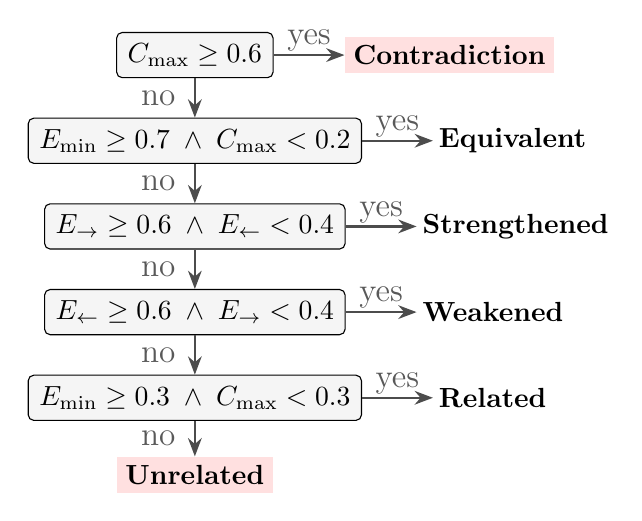
\begin{tikzpicture}[
  test/.style={draw, rounded corners=2pt, fill=gray!8, inner sep=4pt, minimum height=0.55cm},
  cat/.style={font=\bfseries, anchor=west, fill=white, inner sep=2pt},
  drift/.style={font=\bfseries, anchor=west, fill=red!12, inner sep=3pt},
  fall/.style={anchor=east, text=black!65, font=\large},
  yes/.style={above, inner sep=1pt, text=black!65, font=\large},
  >=Stealth, node distance=0.5cm,
]
\node[test] (c1) {$C_{\max} \geq 0.6$};
\node[test, below=of c1] (c2) {$E_{\min} \geq 0.7 \;\wedge\; C_{\max} < 0.2$};
\node[test, below=of c2] (c3) {$E_{\rightarrow} \geq 0.6 \;\wedge\; E_{\leftarrow} < 0.4$};
\node[test, below=of c3] (c4) {$E_{\leftarrow} \geq 0.6 \;\wedge\; E_{\rightarrow} < 0.4$};
\node[test, below=of c4] (c5) {$E_{\min} \geq 0.3 \;\wedge\; C_{\max} < 0.3$};
\node[drift, right=0.9cm of c1.east] (l1) {Contradiction};
\node[cat,   right=0.9cm of c2.east] (l2) {Equivalent};
\node[cat,   right=0.9cm of c3.east] (l3) {Strengthened};
\node[cat,   right=0.9cm of c4.east] (l4) {Weakened};
\node[cat,   right=0.9cm of c5.east] (l5) {Related};
\node[drift, below=0.45cm of c5.south, anchor=north] (l6) {Unrelated};
\foreach \i/\lab in {1/l1, 2/l2, 3/l3, 4/l4, 5/l5} {
  \draw[->, thick, black!70] (c\i.east) -- node[yes] {yes} (\lab);
}
\foreach \i/\j in {1/c2, 2/c3, 3/c4, 4/c5} {
  \draw[->, thick, black!70] (c\i.south) -- node[fall] {no\;} (\j.north);
}
\draw[->, thick, black!70] (c5.south) -- node[fall] {no\;} (l6.north);
\end{tikzpicture}
\end{document}
